%%%%%%%%%%%%%%%%%%%%% {{{
%%Options for presentations (in-class) and handouts (e.g. print).
\documentclass[pdf,9pt]{beamer}


%%%%%%%%%%%%%%%%%%%%%%
%Change this for different slides so it appears in bar
\usepackage{authoraftertitle}
\date{Chapter 5. Vector Space $\R^n$ \\ \S 5-4. Rank of a Matrix}

%%%%%%%%%%%%%%%%%%%%%%
%% Upload common style file
\usepackage{LyryxLAWASlidesStyle}

\begin{document}

%%%%%%%%%%%%%%%%%%%%%%%
%% Title Page and Copyright Common to All Slides

%Title Page
\input frontmatter/titlepage.tex

%LOTS Page
\input frontmatter/lyryxopentexts.tex

%Copyright Page
\input frontmatter/copyright.tex

%%%%%%%%%%%%%%%%%%%%%%%%% }}}
%-------------- start slide -------------------------------%{{{ 2
\begin{frame}[fragile]
   \tableofcontents
\end{frame}
%-------------- end slide -------------------------------%}}}
\section[\textcolor{yellow}{}]{\textcolor{yellow}{Row Space and Column Spaces}}
%-------------- start slide -------------------------------%{{{ 3
\frame{
\frametitle{Row Space and Column Spaces}
\pause
\begin{definitions}
  Let $A$ be an $m\times n$ matrix.
  \begin{itemize}
  \item The \alert{column space of $A$}, denoted \alert{$\col(A)$} is the
    subspace of $\RR^m$ spanned by the columns of $A$.
  \begin{center}
      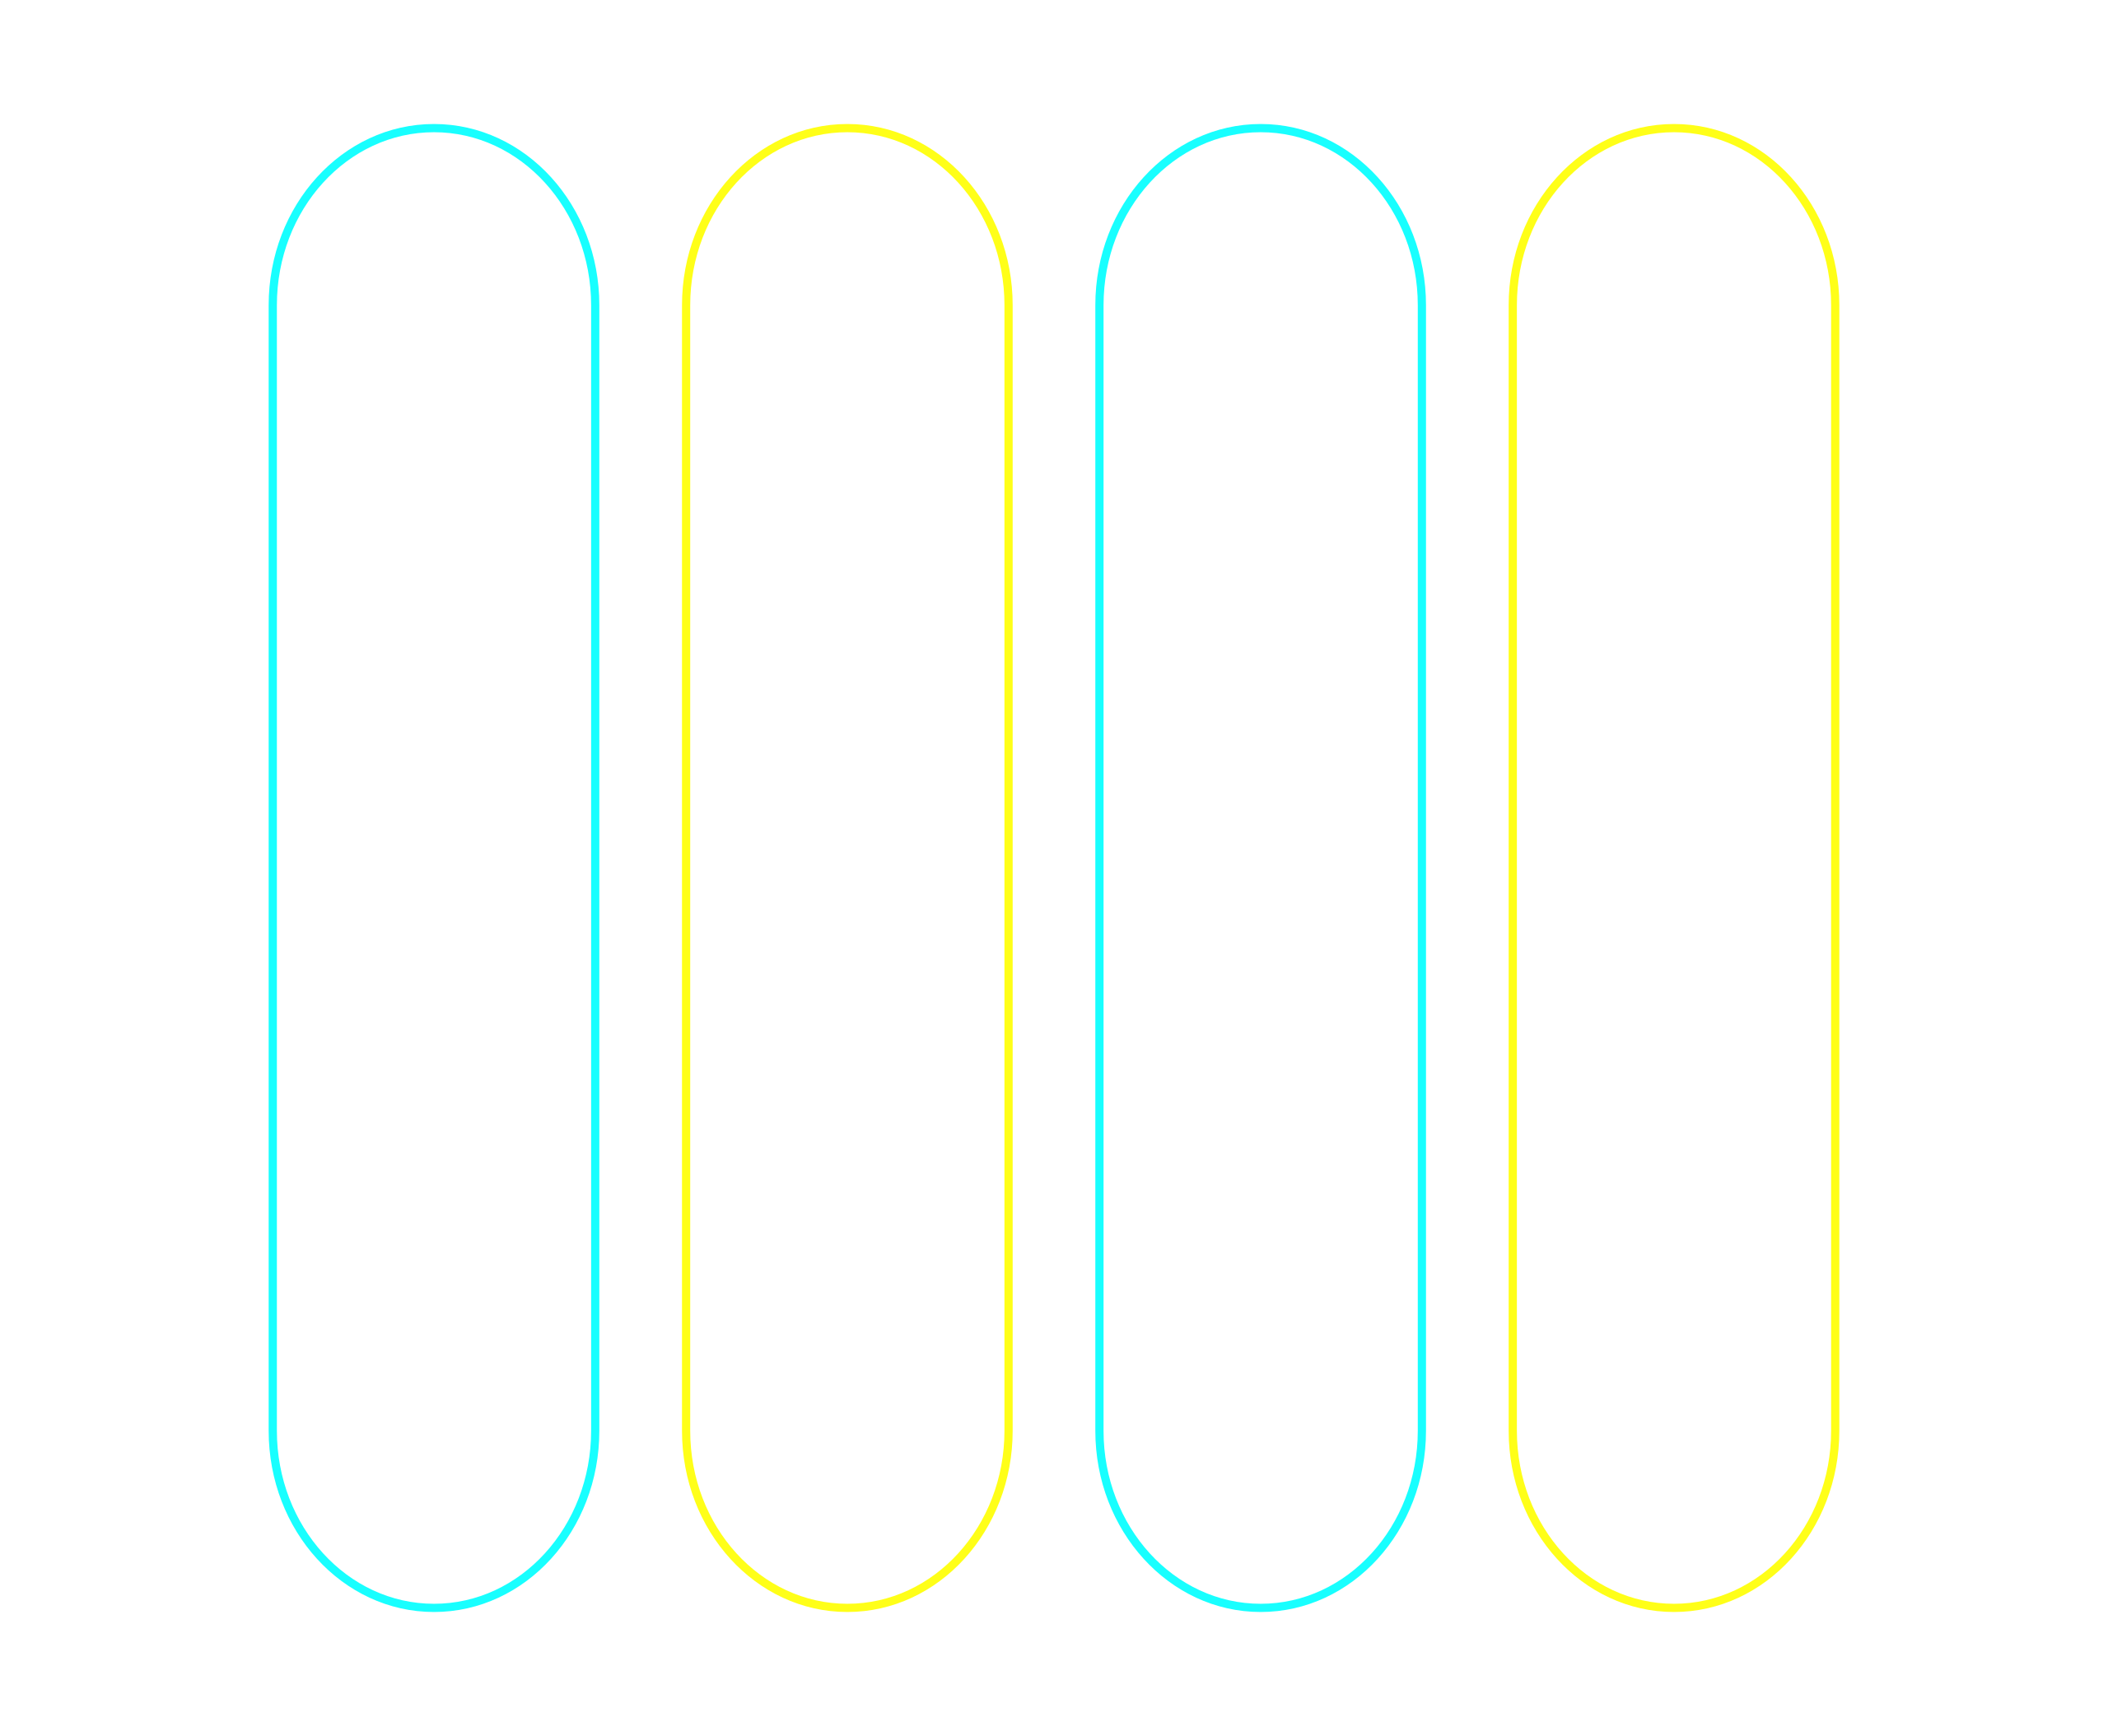
\includegraphics[scale=0.03]{./figures/Matrix_Columns.png}
  \end{center}
  \bigskip
  \pause
  \item The \alert{row space of $A$}, denoted \alert{$\row(A)$} is the
    subspace of $\RR^n$ spanned by the rows of $A$ (or the columns of $A^T$).
  \begin{center}
      
\includegraphics[scale=0.03]{./figures/Matrix_Rows.png}
  \end{center}
  \end{itemize}
\end{definitions}
}
%-------------- end slide -------------------------------%}}}
%-------------- start slide -------------------------------%{{{ 4
\begin{frame}[fragile]
  \begin{emptytitle}
We saw earlier  that
\alert{$\col(A)=\im(A)$}.
  \end{emptytitle}
  \pause
  \vfill
  \begin{remark}[ Notation ]
    Let $A$ and $B$ be $m\times n$ matrices.
    We write \alert{$A\rightarrow B$} if $B$ can be obtained
    from $A$ by a sequence of elementary row (column) operations.
    Note that $A\rightarrow B$ if and only if $B\rightarrow A$.
  \end{remark}
\end{frame}
%-------------- end slide -------------------------------%}}}
%-------------- start slide -------------------------------%{{{ 5
\frame{
\begin{lemma}
  Let $A$ and $B$ be $m\times n$ matrices.
  \begin{enumerate}
    \item If $A\rightarrow B$ by elementary row operations, then $\row(A)=\row(B)$.
    \item If $A\rightarrow B$ by \alert{elementary column operations}, then $\col(A)=\col(B)$.
  \end{enumerate}
\end{lemma}
\pause
\vfill
\begin{proofnoend}
  It suffices to prove only part one, and only for a single row operation. \alert{(Why?)}
  \pause

  Thus let $\vec{r}_1, \vec{r}_2, \ldots, \vec{r}_m$ denote the rows of $A$.
  \pause
  \begin{itemize}
  \item If $B$ is obtained from $A$ by interchanging two rows of $A$, then $A$
    and $B$ have exactly the same rows, so $\row(B)=\row(A)$.
  \end{itemize}
\end{proofnoend}
}
%-------------- end slide -------------------------------%}}}
%-------------- start slide -------------------------------%{{{ 6
\frame{
\begin{proofnoend}[continued]
\begin{itemize}
  \item Suppose $p\neq 0$, and suppose that for some $j$, $1\leq j\leq m$, $B$
    is obtained from $A$ by multiplying row $j$ by $p$.  Then
    \[
      \row(B)=\Span\{ \vec{r}_1, \ldots, p\vec{r}_{j}, \ldots, \vec{r}_m\}.
    \]
    Since
    \[
      \{ \vec{r}_1, \ldots, p\vec{r}_{j}, \ldots, \vec{r}_m\} \subseteq\row(A),
    \]
    it follows that $\row(B)\subseteq\row(A)$.
    \pause
    Conversely, since
    \[ \{ \vec{r}_1, \ldots, \vec{r}_m\}\subseteq\row(B),\]
    it follows that $\row(A)\subseteq\row(B)$.
    Therefore, $\row(B)=\row(A)$.
\end{itemize}
\end{proofnoend}
}
%-------------- end slide -------------------------------%}}}
%-------------- start slide -------------------------------%{{{ 7
\frame{
\begin{proofnoend}[continued]
\begin{itemize}
  \item Suppose $p\neq 0$, and suppose that for some $i$ and $j$, $1\leq
    i,j\leq m$, $B$ is obtained from $A$ by adding $p$ time row $j$ to row $i$.
    Without loss of generality, we may assume $i<j$.
    \pause
    Then
    \[
      \row(B)=\Span\{ \vec{r}_1, \ldots, \vec{r}_{i-1}, \vec{r}_i+p\vec{r}_j, \ldots,\vec{r}_j,\ldots, \vec{r}_m\}.
    \]
    Since
    \[
      \{ \vec{r}_1, \ldots, \vec{r}_{i-1}, \vec{r}_i+p\vec{r}_{j}, \ldots, \vec{r}_m\} \subseteq\row(A),
    \]
    it follows that $\row(B)\subseteq\row(A)$.
    \pause
    Conversely, since
    \[ \{ \vec{r}_1, \ldots, \vec{r}_m\}\subseteq\row(B),\]
    it follows that $\row(A)\subseteq\row(B)$.
    Therefore, $\row(B)=\row(A)$.
\end{itemize}
\myQED\end{proofnoend}
}
%-------------- end slide -------------------------------%}}}
%-------------- start slide -------------------------------%{{{ 8
\frame{
\begin{corollary}
  Let $A$ be an $m\times n$ matrix,
  $U$ an invertible $m\times m$ matrix,
  and $V$ an invertible $n\times n$ matrix.
  Then $\row(UA)=\row(A)$ and $\col(AV)=\col(A)$,
\end{corollary}
\pause
\vfill
\begin{proofnoend}
  Since $U$ is invertible, $U$ is a product of elementary
  matrices, implying that $A\rightarrow UA$ by a sequence of
  elementary row operations.
  By Lemma 2, $\row(UA)=\row(A)$.
  \medskip

  Now consider $AV$:
  $\col(AV)=\row((AV)^T)=\row(V^TA^T)$ and $V^T$ is
  invertible (a matrix is invertible if and only if its
  transpose is invertible).
  It follows from the first part of this Corollary that
  \[ \row(V^TA^T) = \row(A^T).\]
  But $\row(A^T)=\col(A)$, and therefore $\col(AV)=\col(A)$.
  \myQED
\end{proofnoend}
}
%-------------- end slide -------------------------------%}}}
%-------------- start slide -------------------------------%{{{ 9
\frame{
\begin{lemma}
  If $R$ is a row-echelon matrix then
  \begin{enumerate}
    \item the nonzero rows of $R$ are a basis of $\row(R)$;
    \item the columns of $R$ containing the leading ones are a basis of $\col(R)$.
  \end{enumerate}
\end{lemma}
}
%-------------- end slide -------------------------------%}}}
%-------------- start slide -------------------------------%{{{ 10
\begin{frame}[fragile]
\begin{example}
    Let \[
      R=\left[\begin{array}{rrrrrr}
        \alert{1} & \alert{2} & 2 & \alert{-2} & 0  & \alert{0} \\
        0         & \alert{1} & 3 & \alert{1}  & -1 & \alert{2} \\
        0         & 0         & 0 & \alert{1}  & -2 & \alert{5} \\
        0         & 0         & 0 & 0          & 0  & \alert{1} \\
        0         & 0         & 0 & 0          & 0  & 0
    \end{array}\right].
  \]
  \begin{enumerate}
    \item Since the nonzero rows of $R$ are linearly independent, they form a
      basis of $\row(R)$.
	\pause
	% \vspace*{-.06in}
    \item Let $B=\{ \vec{e}_1, \vec{e}_2, \vec{e}_3, \vec{e}_4\}\subseteq
      \RR^5$.  Then $B$ is linearly independent and spans $\col(R)$, and thus
      is a basis of $\col(R)$.  \alert{This tells us that $\dim(\col(R))=4$.}
      Now let $X$ denote the set of columns of $R$ that contain the leading
      ones.
	\pause
    Then $X$ is a linearly independent subset of $\col(R)$ with
    $4=\dim(\col(R))$ vectors.
    It follows that $X$ spans $\col(R)$, and therefore is a basis
    of $\col(R)$.
\end{enumerate}
\end{example}
\end{frame}
%-------------- end slide -------------------------------%}}}
%-------------- start slide -------------------------------%{{{ 11
\frame{
\begin{problem}
  Find a basis of
  $U=\Span \left\{
  \left[\begin{array}{r} 1 \\ -1 \\ 0 \\ 3 \end{array}\right],
  \left[\begin{array}{r} 2 \\ 1 \\ 5 \\ 1 \end{array}\right],
  \left[\begin{array}{r} 4 \\ -1 \\ 5 \\ 7 \end{array}\right]\right\}$
  and find $\dim(U)$.
\end{problem}
\pause
\begin{solution}
  Let $A$ the the $3\times 4$ matrix whose \alert{rows} are the
  three columns listed.
  Then $U=\row(A)$, so it suffices to find a basis of $\row(A)$.
  \[ A=
  \left[\begin{array}{rrrr}
      1 & -1 & 0 & 3 \\
      2 & 1  & 5 & 1 \\
      4 & -1 & 5 & 7
  \end{array}\right].\]
  Find $R$, a row-echelon form of $A$.
  Then the \alert{nonzero rows of $R$} are a basis of $\row(R)$.
  Since $\row(A)=\row(R)$, the nonzero rows of $R$ are a basis
  of $\row(A)$.
\end{solution}
}
%-------------- end slide -------------------------------%}}}
%-------------- start slide -------------------------------%{{{ 12
\frame{
    \begin{solution}[continued]
    \[ \left[\begin{array}{rrrr}
    1 & -1 & 0 & 3 \\
    2 & 1 & 5 & 1  \\
    4 & -1 & 5 & 7 \end{array}\right]
    \rightarrow
    \left[\begin{array}{rrrr}
    1 & -1 & 0 & 3 \\
    0 & 1 & 5/3 & -5/3  \\
    0 & 0 & 0 & 0 \end{array}\right].\]
    Therefore,
    $B=\left\{
    \left[\begin{array}{r} 1 \\ -1 \\ 0 \\ 3 \end{array}\right],
    \left[\begin{array}{r} 0 \\ 3 \\ 5 \\ -5 \end{array}\right]
    \right\}$ is a basis of $U$ and $\dim(U)=2$.
\end{solution}
\pause
\begin{solution}[Another solution -- usually more work.]
Take a linear combination of the three given vectors and set it
equal to $\vec{0}_4$.
If the vectors are independent, then they form a basis of $U$.
Otherwise, delete vectors to cut the given set of vectors
down to a basis.
\end{solution}
}
%-------------- end slide -------------------------------%}}}
\section[\textcolor{yellow}{}]{\textcolor{yellow}{The Rank Theorem}}
%-------------- start slide -------------------------------%{{{ 13
\begin{frame}[fragile]
\frametitle{The Rank Theorem}
\pause
    \[ \dim(\row(A))=\dim(\col(A))=\rank(A)\]
\end{frame}
%-------------- end slide -------------------------------%}}}
%-------------- start slide -------------------------------%{{{ 14
\frame{
\begin{remark}
    Recall that $\rank(A)$ is defined to be the nonzero rows in the row echelon form of $A$.
    From what we just learned, the \alert{rank of $A$} can be equivalently defined as \alert{$\rank(A)=\dim(\row(A))$.}
\end{remark}
\pause
\begin{theorem}[Rank Theorem]
Let $A=\left[\begin{array}{cccc} \vec{A_1} & \vec{A_2} & \cdots &
\vec{A_n}\end{array}\right]$
be an $m\times n$ matrix with columns $\{ \vec{A_1}, \vec{A_2},
\ldots, \vec{A_n}\}$,
and suppose that $\rank(A)=r$.
Then
\[ \dim(\row(A))=\dim(\col(A))=r.\]
Furthermore, if $R$ is a row-echelon form of $A$ then
\begin{enumerate}
\item the $r$ nonzero rows of $R$ are a basis of $\row(A)$;
\item if $S=\{\vec{A}_{j_1}, \vec{A}_{j_2}, \ldots, \vec{A}_{j_r}\}$
are the $r$ columns of $A$ corresponding to the
columns of $R$ containing leading ones, then $S$ is basis
of $\col(A)$.
\end{enumerate}
\end{theorem}
}
%-------------- end slide -------------------------------%}}}
%-------------- start slide -------------------------------%{{{ 15
\frame{
    \begin{problem}
        For the following matrix $A$, find $\rank(A)$ and bases for $\row(A)$ and $\col(A)$.
        \[ A= \left[\begin{array}{rrrr}
                2 & -4 & 6 & 8 \\
                2 & -1 & 3 & 2 \\
                4 & -5 & 9 & 10 \\
                0 & -1 & 1 & 2
        \end{array}\right].\]
    \end{problem}
    \pause
    \begin{solution}
        \[ \left[\begin{array}{rrrr}
                2 & -4 & 6 & 8 \\
                2 & -1 & 3 & 2 \\
                4 & -5 & 9 & 10 \\
                0 & -1 & 1 & 2
        \end{array}\right]
        \rightarrow
        \left[\begin{array}{rrrr}
                1 & -2 & 3 & 4 \\
                0 & 1 & -1 & -2 \\
                0 & 0 & 0 & 0 \\
                0 & 0 & 0 & 0
        \end{array}\right]
    \]
    \pause
    \begin{itemize}
        \item $\rank(A)=2$.
            \pause
        \item
            $\{
                \left[\begin{array}{rrrr} 1 & -2 & 3 & 4 \end{array}\right],
                \left[\begin{array}{rrrr} 0 & -1 & -1 & 2 \end{array}\right]
            \}$
            is a basis of $\row(A)$.
            \pause
        \item
            $\left\{
                \left[\begin{array}{r} 2  \\ 2  \\ 4  \\ 0  \end{array}\right],
                \left[\begin{array}{r} -4 \\ -1 \\ -5 \\ -1 \end{array}\right]
            \right\}$
            is a basis of $\col(A)$.\myQED
    \end{itemize}
\end{solution}
}
%-------------- end slide -------------------------------%}}}
%-------------- start slide -------------------------------%{{{ 16
\frame{
    \begin{problem}[revisited]
      Find a basis of
      $U=\Span \left\{
          \left[\begin{array}{r} 1 \\ -1 \\ 0 \\ 3 \end{array}\right],
          \left[\begin{array}{r} 2 \\ 1  \\ 5 \\ 1 \end{array}\right],
          \left[\begin{array}{r} 4 \\ -1 \\ 5 \\ 7 \end{array}\right]
      \right\}$
      and find $\dim(U)$.
    \end{problem}
    \pause
    \vfill
    \begin{solution}
      Let $A$ denote the matrix whose columns are the three vectors
      listed, and let $R$ denote a row-echelon form of $A$.
      Then
      \[ A=\left[\begin{array}{rrr}
            1  & 2 & 4  \\
            -1 & 1 & -1 \\
            0  & 5 & 5  \\
            3  & 1 & 7
      \end{array}\right]
      \rightarrow
      \left[\begin{array}{rrr}
            1 & 2 & 4 \\
            0 & 1 & 1 \\
            0 & 0 & 0 \\
            0 & 0 & 0
      \end{array}\right] = R.  \]
      By the Rank Theorem,
      $\left\{
          \left[\begin{array}{r} 1 \\ -1 \\ 0 \\ 3 \end{array}\right],
          \left[\begin{array}{r} 2 \\ 1  \\ 5 \\ 1 \end{array}\right]
      \right\}$
      is a basis of $U=\col(A)$, so $\dim(U)=2$. \myQED
    \end{solution}
	\bigskip
	\begin{center}
	    \alert{Compare this to the basis found earlier.}
	\end{center}
}
%-------------- end slide -------------------------------%}}}
%-------------- start slide -------------------------------%{{{ 17
\frame{
\begin{corollary}
\begin{enumerate}
    \item For any matrix $A$, $\rank(A)=\rank(A^T)$.
    \item For any $m\times n$ matrix $A$, $\rank(A)\leq m$ and $\rank(A)\leq n$.
    \item Let $A$ be an $m\times n$ matrix.
        If $U$ and $V$ are invertible matrices (of sizes $m\times m$ and
        $n\times n$, respectively), then
    \[ \rank(A)=\rank(UA)=\rank(AV).\]
\end{enumerate}
\end{corollary}
}
%-------------- end slide -------------------------------%}}}
%-------------- start slide -------------------------------%{{{ 18
\frame{
\begin{lemma}
  Let $A$ be an $m\times n$ matrix, $U$ a $p\times m$ matrix, and
  $V$ an $n\times q$ matrix.
  \begin{enumerate}
      \item $\col(AV)\subseteq \col(A)$ with equality if $VV'=I_n$ for some $V'$.
      \item $\row(UA)\subseteq \row(A)$ with equality if $U'U=I_m$ for some $U'$.
  \end{enumerate}
\end{lemma}
\pause
\vfill
\begin{proofnoend}
(1) Write $V=\left[\begin{array}{cccc} \vec{v}_1 & \vec{v}_2 & \cdots & \vec{v}_q\end{array}\right]$,
    where $\vec{v}_j$ denotes column $j$ of $V$, $1\leq j\leq q$.
    Then
    $AV = \left[\begin{array}{cccc} A\vec{v}_1 & A\vec{v}_2 & \cdots & A\vec{v}_q\end{array}\right]$,
    where $A\vec{v}_j$ is column $j$ of $AV$.
    By the definition of matrix-vector multiplication, $A\vec{v}_j$ is
    a linear combination of the columns of $A$, and thus
    $A\vec{v}_j\in \col(A)$ for each $j$.
    Since $A\vec{v}_1, A\vec{v}_2, \ldots, A\vec{v}_q\in \col(A)$,
    \[ \Span \{ A\vec{v}_1, A\vec{v}_2, \ldots, A\vec{v}_q\} \subseteq \col(A),\]
    i.e., $\col (AV)\subseteq \col(A)$.
    \pause
    If for some $V'$ we have $VV'=I_n$, then
    \begin{align*}
	\col(A) = \col(AVV')\subseteq \col(AV) \subseteq \col(A).
    \end{align*}
    \bigskip
    \pause
(2) This can be proved by part (1) and the fact that $\row (A) =\col(A^T)$.
    \myQED
\end{proofnoend}
}
%-------------- end slide -------------------------------%}}}
\section[\textcolor{yellow}{}]{\textcolor{yellow}{Rank-Nullity Theorem}}
%-------------- start slide -------------------------------%{{{ 19
\begin{frame}[fragile]
\frametitle{Rank-Nullity Theorem}
\pause
\begin{center}
    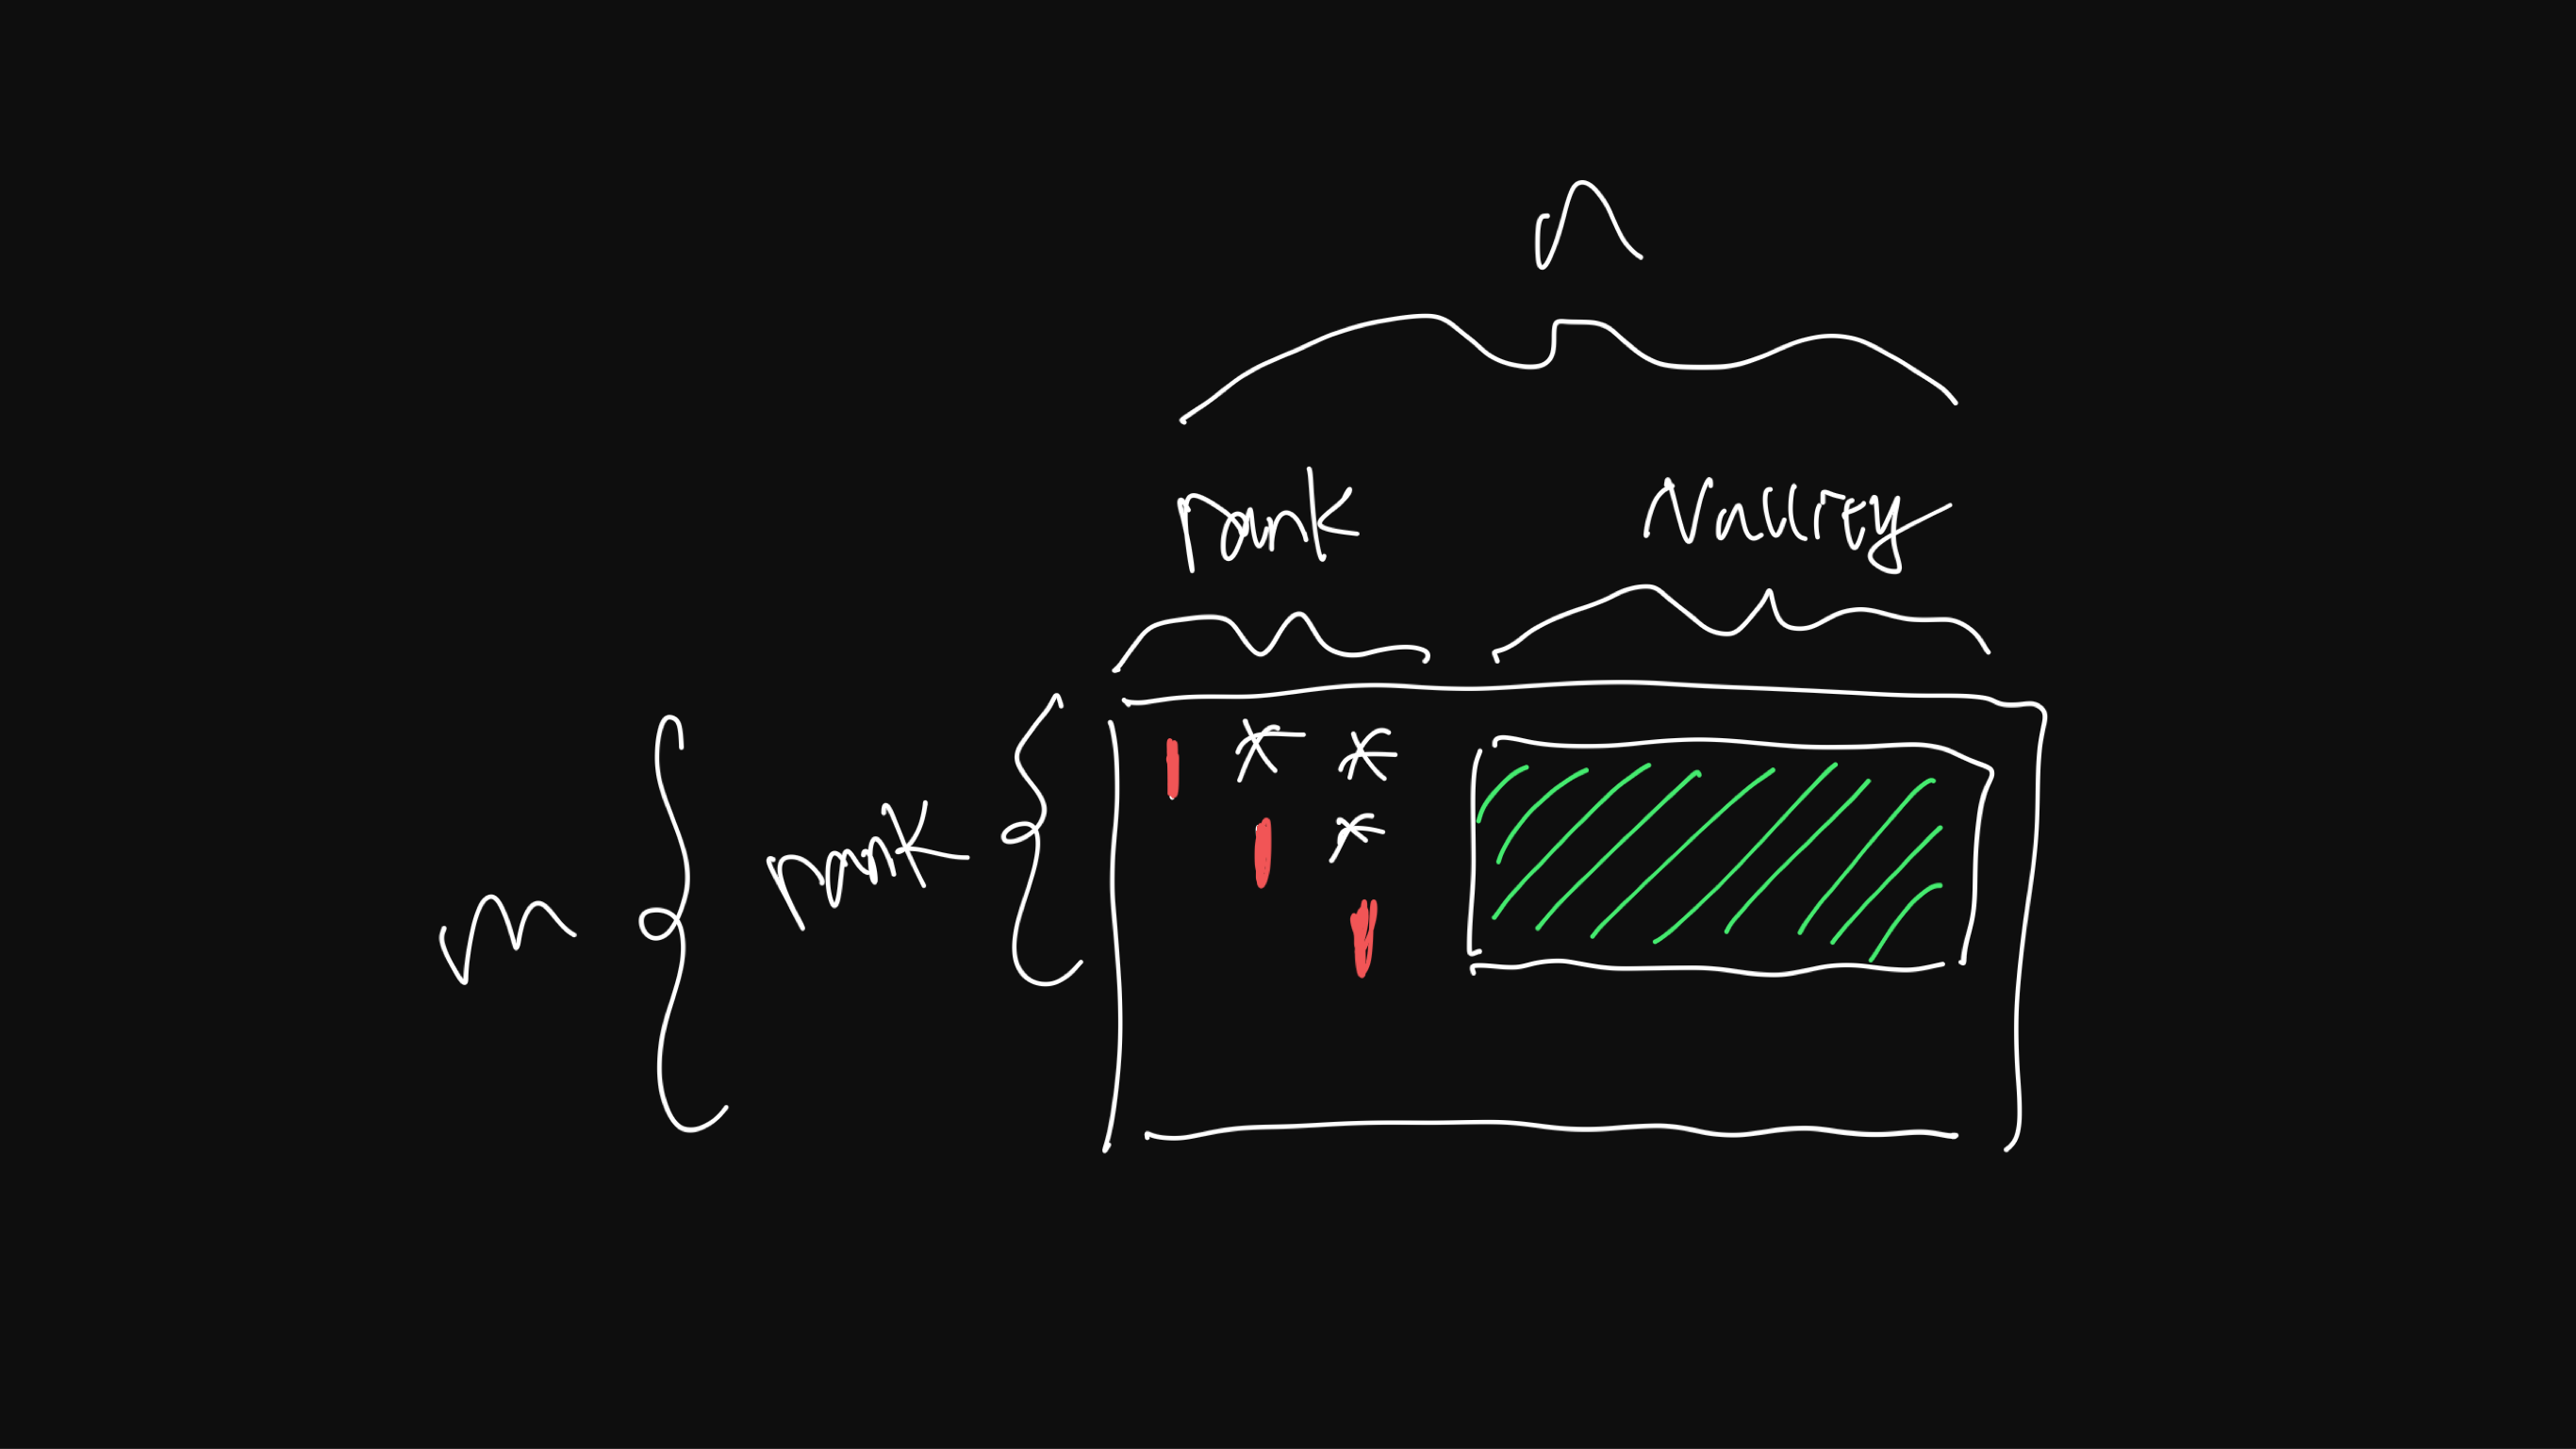
\includegraphics[scale=0.1]{./figures/Rank_Nullity_Illustrate.png}
\end{center}
\end{frame}
%-------------- end slide -------------------------------%}}}
%-------------- start slide -------------------------------%{{{ 20
\frame{
\begin{theorem}[Rank-Nullity Theorem]
Let $A$ denote an $m\times n$ matrix of rank $r$.  Then
% \vspace*{-.1in}
\begin{enumerate}
    \item The $n-r$ basic solutions to the system $A\vec{x}=\vec{0}_m$ provided by the Gaussian algorithm are a basis of
        $\nul(A)$, so
        \begin{align*}
          \dim(\nul(A))=n-r.
        \end{align*}
    \item The rank theorem provides a basis of $\im(A)=\col(A)$, and $\dim(\im(A))=r$.
\end{enumerate}
\end{theorem}
\pause
\vfill
\begin{remark}[Common notation]
    The nullspace $A$ is also called kernel space of $A$, written as $\text{ker}(A)$, i.e., $\text{ker}(A) = \nul(A)$.
    Usually, the \alert{nullity} of $A$ is defined to be
    \begin{align*}
      \text{Nullity}(A)=\dim(\nul(A)) = \dim(\text{ker}(A))
    \end{align*}
\end{remark}
}
%-------------- end slide -------------------------------%}}}
%-------------- start slide -------------------------------%{{{ 21
\begin{frame}[fragile]
    \begin{emptytitle}
       Let $T: V\mapsto W$ be the linear map from space $V$ to $W$.
       Suppose $V=\R^n$ and $W=\R^m$ and let $A$ be the induced matrix.
    \end{emptytitle}
    \vfill
   \begin{emptytitle}
    \begin{align*}
        \begin{array}{ccccc}
          \text{Rank}(T) & + & \text{Nullity}(T)   & = & \dim(V)    \\ [0.5em]
          |  |           &   & |  |                &   & |  |       \\ [0.5em]
          \text{Rank}(A) &   & \text{Nullity}(A)   &   & \dim(\R^n) \\ [0.5em]
          |  |           &   & |  |                &   & |  |       \\ [0.5em]
          \dim(\im(A))   &   & \dim(\nul(A))       &   & n          \\ [0.5em]
                ||       &   & |  |                &   &            \\ [0.5em]
                 r       &   & \dim(\text{ker}(A)) &   &            \\ [0.5em]
        \end{array}
    \end{align*}
   \end{emptytitle}
\end{frame}
%-------------- end slide -------------------------------%}}}
%-------------- start slide -------------------------------%{{{ 22
\begin{frame}[fragile]
   \begin{center}
       
\includegraphics[scale=0.08]{./figures/Rank-nullity.png}
   \end{center}
\end{frame}
%-------------- end slide -------------------------------%}}}
%-------------- start slide -------------------------------%{{{ 23
\begin{frame}[fragile]
\begin{proofnoend}[Outline]
% \vspace*{-.03in}
    \begin{itemize}
      \item We have already seen that $\nul(A)$
          is spanned by any set of basic solutions to $A\vec{x}=\vec{0}_m$,
          so it is enough to prove that $\dim(\nul(A))=n-r$, which will implies that
	  the set of basic solutions is independent, hence this set forms a basis.
      \item Suppose $\{\vec{x}_1, \vec{x}_2, \ldots, \vec{x}_k\}$ is a basis of  $\nul(A)$
      \item Extend $\{\vec{x}_1, \vec{x}_2, \ldots, \vec{x}_k\}$ to a basis
          $\{\vec{x}_1, \vec{x}_2, \ldots, \vec{x}_k,\ldots \vec{x}_n\}$ of $\RR^n$.
      \item Consider the set $\{A\vec{x}_1, A\vec{x}_2, \ldots, A\vec{x}_k,\ldots A\vec{x}_n\}\subseteq \R^m$
      \item Then
          $A\vec{x}_j = \vec{0}_m$ for $1\leq j\leq k$
          since $\vec{x}_1, \ldots, \vec{x}_k\in\nul(A)$.
      \item To complete the proof, show
          $S=\{ A\vec{x}_{k+1},\ldots A\vec{x}_n\}$ is a basis of $\im(A)$,
	  by showing that (exercise!)\\
      (1)  $S$ is independent\\
      (2) $S$ spans $\im(A)$
      \item Since $\im(A)=\col(A)$, $\dim(\im(A))=r$, implying
          $n-k=r$. Hence $k=n-r$.  \myQED
    \end{itemize}
\end{proofnoend}

\end{frame}
%-------------- end slide -------------------------------%}}}
%-------------- start slide -------------------------------%{{{ 24


\frame{
\begin{problem}
  For the following matrix $A$, find
  bases for $\nul(A)$ and $\im(A)$, and find their dimensions.
  \[ A= \left[\begin{array}{rrrr}
    2 & -4 & 6 & 8 \\
    2 & -1 & 3 & 2 \\
    4 & -5 & 9 & 10 \\
    0 & -1 & 1 & 2
  \end{array}\right].\]
\end{problem}
}
%-------------- end slide -------------------------------%}}}
%-------------- start slide -------------------------------%{{{ 25
\begin{frame}[fragile]
\begin{solution}
    Find the basic solutions to $A\vec{x}=\vec{0}_4$.
    \[
      \left[\begin{array}{rrrr|r}
        2 & -4 & 6 & 8 & 0 \\
        2 & -1 & 3 & 2 & 0 \\
        4 & -5 & 9 & 10 & 0 \\
        0 & -1 & 1 & 2 & 0
      \end{array}\right]
      \rightarrow
      \left[\begin{array}{rrrr|r}
        1 & -2 & 3 & 4 & 0 \\
        0 & 1 & -1 & -2 & 0 \\
        0 & 0 & 0 & 0 & 0 \\
        0 & 0 & 0 & 0 & 0
      \end{array}\right].
    \]
    Hence,
    \begin{align*}
      \vec{x}=\left[\begin{array}{c} -s \\ s+2t \\ s \\ t \end{array}\right]\quad s,t\in\RR.
    \end{align*}
    \pause
    Therefore,
    \vspace{-1em}
    \[
      \left\{
          \left[\begin{array}{r} -1 \\ 1 \\ 1 \\ 0 \end{array}\right],
          \left[\begin{array}{r} 0 \\ 2 \\ 0 \\ 1 \end{array}\right]
      \right\} \quad\text{and}\quad
      \left\{
          \left[\begin{array}{r} 2 \\ 2 \\ 4 \\ 0 \end{array}\right],
          \left[\begin{array}{r} -4 \\ -1 \\ -5 \\ -1 \end{array}\right]
      \right\}
    \]
    are bases of $\nul(A)$ and $\im(A)$, respectively, so
    \[
      \dim(\nul(A))=2 \quad\text{and}\quad \dim(\im(A))=2.
    \]
    \myQED
\end{solution}
\end{frame}
%-------------- end slide -------------------------------%}}}
%-------------- start slide -------------------------------%{{{ 26
\frame{
\begin{problem}
Can a $5\times 6$ matrix have independent columns?  Independent rows?
Justify your answer.
\end{problem}
\pause
\vfill
\begin{solution}
    The rank of the matrix is at most five;
    since there are six columns,
    \alert{the columns can not be independent}.
    However, the rows could be independent:
    \pause
    take a $5\times 6$ matrix whose first five columns are
    the columns of the $5\times 5$ identity matrix.
\end{solution}
}
%-------------- end slide -------------------------------%}}}
%-------------- start slide -------------------------------%{{{ 27
\frame{
\begin{problem}
    Let $A$ be an $m\times n$ matrix with $\rank(A)=m$.
    Prove that $m\leq n$.
\end{problem}
\pause
\vfill
\begin{proofnoend}
    As a consequence of the Rank Theorem, we have
    \[ \rank(A)\leq m \quad\text{and}\quad\rank(A)\leq n.\]
    Since $\rank(A)=m$, it follows that $m\leq n$.
    \myQED
\end{proofnoend}
}
%-------------- end slide -------------------------------%}}}
%-------------- start slide -------------------------------%{{{ 28
\frame{
\begin{problem}
    Let $A$ be an $5\times 9$ matrix.
    Is it possible that $\dim(\nul(A))=3$?
    Justify your answer.
\end{problem}
\pause
\vfill
\begin{solution}
    As a consequence of the Rank Theorem, we have
    $\rank(A)\leq 5$,
    so $\dim(\im(A))\leq 5$.
    Since $\dim(\nul(A))= 9-\dim(\im(A))$, it follows that
    \[ \dim(\nul(A)) \geq 9 - 5 = 4.\]
    Therefore, it is not possible that $\dim(\nul(A))=3$.
    \myQED
\end{solution}
}
%-------------- end slide -------------------------------%}}}
\section[\textcolor{yellow}{}]{\textcolor{yellow}{Full Rank Cases}}
%-------------- start slide -------------------------------%{{{ 29
\frame{
\frametitle{Full Rank Cases}
\pause
\begin{theorem}
    Let $A$ be an $m\times n$ matrix.
    The following are equivalent.
    \pause
    \begin{enumerate}
        \item $\rank(A)=n$.  \pause
        \item $\row(A)=\RR^n$, i.e., the rows of $A$ span $\RR^n$.  \pause
        \item The columns of $A$ are independent in $\RR^m$.  \pause
        \item The $n\times n$ matrix $A^TA$ is invertible.  \pause
        \item There exists and $n\times m$ matrix $C$ so that $CA=I_n$.  \pause
        \item If $A\vec{x}=\vec{0}_m$ for some $\vec{x}\in\RR^n$, then $\vec{x}=\vec{0}_n$.
    \end{enumerate}
\end{theorem}
}
%-------------- end slide -------------------------------%}}}
%-------------- start slide -------------------------------%{{{ 30
\frame{
\begin{theorem}
    Let $A$ be an $m\times n$ matrix.
    The following are equivalent.
    \pause
    \begin{enumerate}
        \item $\rank(A)=m$.
        \pause
        \item $\col(A)=\RR^m$, i.e., the columns of $A$ span $\RR^m$.  \pause
        \item The rows of $A$ are independent in $\RR^n$.  \pause
        \item The $m\times m$ matrix $AA^T$ is invertible.  \pause
        \item There exists and $n\times m$ matrix $C$ so that $AC=I_m$.  \pause
        \item The system $A\vec{x}=\vec{b}$ is consistent for every $\vec{b}\in\RR^m$.
    \end{enumerate}
\end{theorem}
}
%-------------- end slide -------------------------------%}}}
%-------------- start slide -------------------------------%{{{ 31
\begin{frame}[fragile]
   \begin{problem}
       Let $\vec{x}=(x_1,\cdots,x_k)^T\in \R^k$.
       Show that the following matrix is invertible if and only if $\{x_i,i=1,\cdots, k\}$ are not all equal:
       \begin{align*}
	   \begin{pmatrix}
	   k & x_1+\cdots+x_k\cr
	   x_1+\cdots+x_k &  \Norm{x}^2
       \end{pmatrix}
       \end{align*}
   \end{problem}
   \vfill
   \pause
   \begin{solution}
      Notice that 
       \begin{align*}
	   \begin{pmatrix}
	   k & x_1+\cdots+x_k\cr
	   x_1+\cdots+x_k &  \Norm{x}^2
       \end{pmatrix} = A^T A
       \end{align*}
       with 
       \begin{align*}
       A =     
       \begin{bmatrix} 
	1      & x_1\cr
	1      & x_2\cr
	\vdots & \vdots\cr
	1      & x_k\cr
       \end{bmatrix}.
       \end{align*}
       Now $A^TA$ is invertible  iff the two columns of $A$ are independent iff  $\{x_i,i=1,\cdots, k\}$ are not all equal.
       \myQED
   \end{solution}
\end{frame}
%-------------- end slide -------------------------------%}}}
\end{document}
